\documentclass[../appunti-analisi.tex]{subfiles}

\begin{document}

\section{Lezione 23}

\subsection{Ottimizzazione Vincolata}

\subsubsection{Metodo di parametrizzazione} 

Ricerca di estremo minimo o massimo per la $f(x,y)$ quando i punti $(x,y) \in A$ sono soggetti a un vincolo espresso da un'equazione:

\[
    g(x,y) = k
\]

\[
    g(x,y) -k = 0
\]

con $g \in \mathbb{C}^{1}$ e g soggetto a:

\[
    V= \{(x,y) \in A; g(x,y) =k\}
\]

Questo metodo utilizza la parametrizzazione della curva del vincolo che permette di trovare il minimo/massimo tramite ponendo:

\[
    F'(t) = 0
\]

quindi risolvendo il problema come se fosse analisi I.

\newpage

\textbf{Esempio} 

\[
    V = \{(x,y) \in \mathbb{R}^{2}; x^{2}+y^{2}=4\}
\]

\begin{center}
\begin{tikzpicture}[line width=1pt]
  \draw (0,0) circle (1.5cm);
  \draw[->,ultra thick] (-5,0)--(5,0) node[right]{$x$};
  \draw[->,ultra thick] (0,-5)--(0,5) node[above]{$y$};

  % etichette per le coordinate
  \node[above] at (2,0) {(2,0)};
  \node[below] at (-2,0) {(-2,0)};
  \node[right] at (0,2) {(0,2)};
  \node[left] at (0,-2) {(0,-2)};
\end{tikzpicture}
\end{center}

Problema di minimo e massimo di $f$ rispetto al vincolo $V$.

Se nel vincolo riesco a esplicitare una variabile in funzione dell'altra $\rightarrow y=y(x)$.

Se $y=y(x),g(x,y) = k$ diventa $g(x,y(x))=k$ funziona di \textbf{una} sola variabile.

Infatti nell'esempio di prima:

\[
    x^{2}+y^{2} = 4
\]

\[
    V = \gamma([0,2\pi])
\]

\[
    \gamma =
        \begin{cases}
            x=2 \cos t\\
               y= 2 \sin t
        \end{cases}\,.
\]

diventa:

\[
    x^{2}+y^{2} = 4 \cos ^{2} t + 4 \sin ^{2} t = 4 ( \cos ^{2} t + \sin ^{2} t) =4
\]

\subsubsection{Metodo dei moltiplicatori di Lagrange}

Questo è il metodo che pone delle condizioni affinché il le curve di livello della mia funzione ``bacino'' il vincolo, in questo modo, i punti trovati sono dei candidati minimi/massimi.

\textbf{Esempio} 

Cerchiamo il massimo della funzione $f(x,y) = xy$ quando $(x,y) \in \mathbb{R}^{2}$ si muove su:

\[
    V= \{(x,y) \in \mathbb{R}^{2};\underbrace{ x^{2}+y^{2}=1}_\text{$g(x,y) = k$} x \ge 0, y \ge 0\}
\]

Quindi sto restringendo il dominio della mia funzione a questo cerchio.

\textbf{Osservazione} 

Sia $f$ che $g \in \mathbb{C}^{1}(\mathbb{R}^{2})$

Quello che faccio è disegnare gli insiemi di livello della funzione $f$:

\[
    E_c = \{(x,y) \in \mathbb{R}^{2}, \underbrace{xy = c}_\text{la funzione equivale a una costante}, c \in \mathbb{R}\}
\]

Voglio trovare il valore massimo di $f$ in $V$ e dunque devo trovare il valore di $c$ per cui l'insieme di livello interseca il vincolo $V$.


\begin{figure}[ht]
    \incfig{insieme-di-livello-lagrange}
    \caption{insieme di livello Lagrange}
    \label{fig:insieme-di-livello-lagrange}
\end{figure}

Nel punto rosso in figura \ref{fig:insieme-di-livello-lagrange} chiamato $P_0$ gli insiemi $E_c$ e $V$ hanno la stessa retta tangente.

Quindi si ha per $xy = \frac{1}{2}$:

\[
P_0 = ( \underbrace{\frac{\sqrt{2}}{2}, \frac{\sqrt{2}}{2}}_\text{per avere $c= \frac{1}{2}$})
\]

La curva di livello $xy=\frac{1}{2}$ è tangente al vincolo $P_0$.

Quindi $\nabla f(x_0,y_0)$ è \textbf{ortogonale} alla linea di livello $E_c$.

Supponiamo $E_c \subset \mathbb{R}^{2}$ [l'insieme di livello c della $f(x,y)$] sia il sostegno di una curva piana regolare, dunque $E_c = \gamma([a,b])$ con:

\[
    \gamma(t) = (\gamma_1(t), \gamma_2(t))
\]

allora la funzione composta:

\[
    F(t) = (f \circ \gamma) (t) = f(\gamma(t))
\]

è uguale a $c$. Poniamo:

\[
    F'(t)=0
\]

quindi:

\[
    F'(t) \overset{\text{regola della catena}}{=} \langle \nabla f(\gamma(t)), \gamma'(t) \rangle = 0
\]

questa è la \textbf{condizione geometrica} (sono vettori perpendicolari, come in fisica se l'angolo è 90 allora il prodotto scalare fa 0).

Il gradiente è, in ogni punto, perpendicolare al vettore tangente all'insieme di livello $f(x,y) = c$ quando questi ($E_c$) è il sostegno di una curva regolare.

Si ha poi che il gradiente $\nabla g(x_0,y_0)$ è ortogonale all'insieme $g(x,y) = k$ (ossia il vincolo).


La retta tangente al vincolo (espresso da $g$) ci fornisce la direzione $\vec{v}$ in cui $g=k$ ($g(x,y) -k=0$). La derivata direzionale:

\[
    D_{\vec{v}} g(x_0,y_0) = \langle \nabla g(x_0,y_0), \vec{v} \rangle \overset{\text{visto che $g$ costantemente $=k$}}{=} 0 \implies \nabla g(x_0,y_0) \perp \vec{v}
\]

e dunque i due vettori $\nabla f(x_0,y_0)$ e $\nabla g(x_0,y_0)$ sono paralleli quindi:

\[
\exists \lambda_0 \in \mathbb{R}: \nabla f(x_0,y_0) = \lambda_0 \nabla g(x_0,y_0)
\]

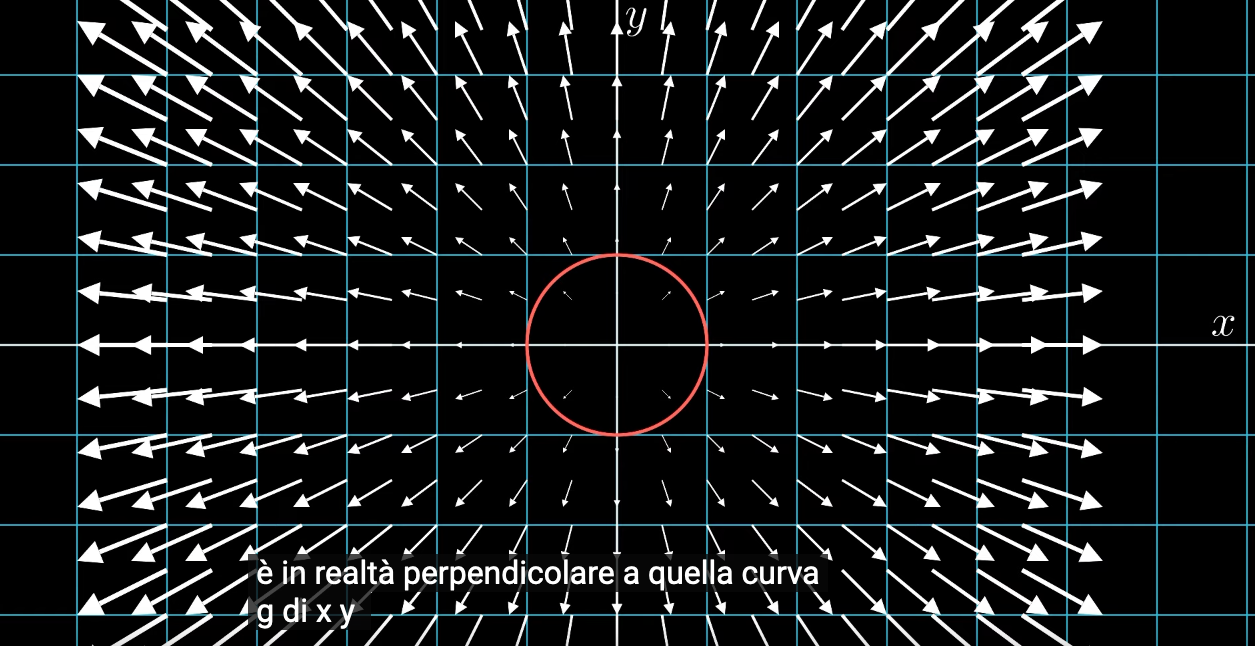
\includegraphics[width=\textwidth]{gradiente-curva}

\begin{center}
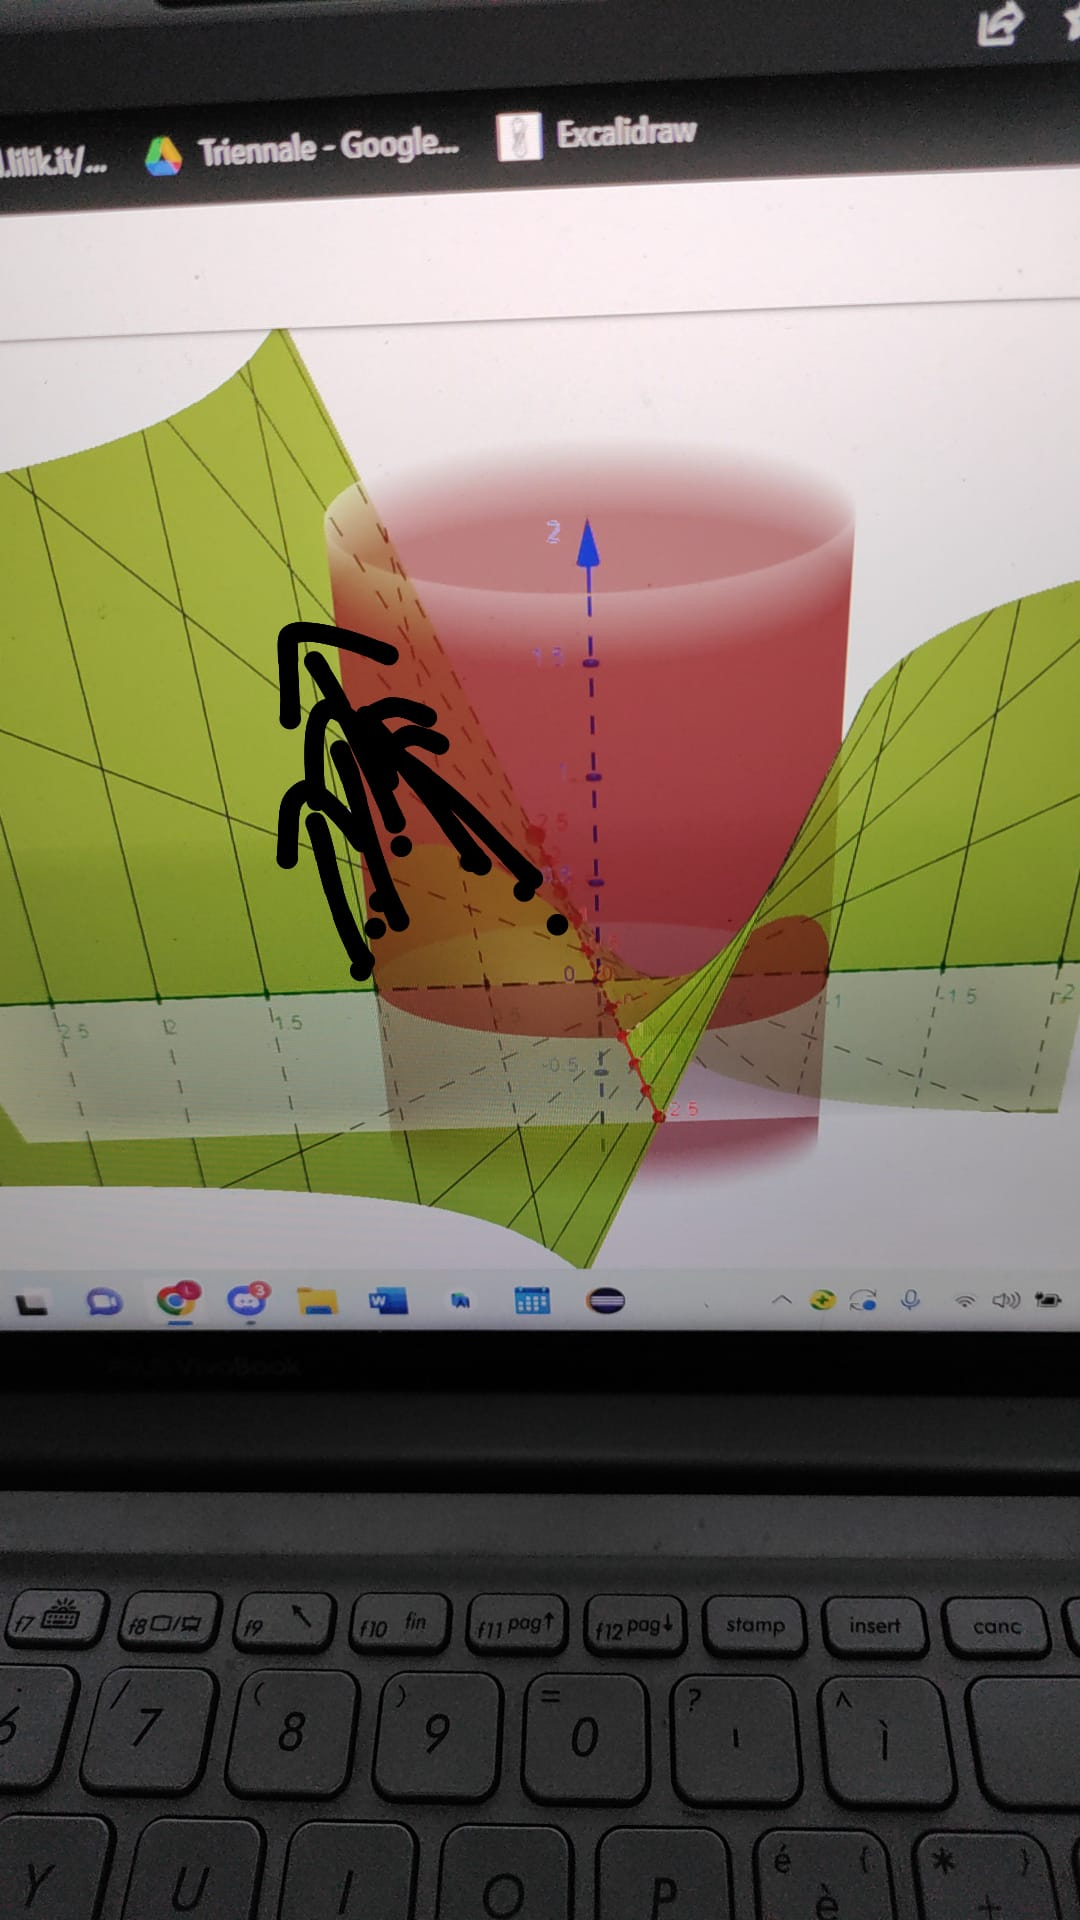
\includegraphics[scale=0.2]{vettori-gradiente}
\end{center}

\newpage

\teorema{Moltiplicatori di Lagrange}{ Supponiamo che $f,g \in \mathbb{C}^{1}(A)$ dove $A \subseteq \mathbb{R}^{2}$ aperto.

    Se $(x_0,y_0) \in A$ è un punto di estremo (minimo o massimo) per la $f$ nell'insieme $V$ ($(x_0,y_0)$ è punto di estremo vincolato):

    \[
        V=\{(x,y) \in A, g(x,y) = k\}
    \]

    e vale anche:

    \[
        \underbrace{\nabla g(x_0,y_0) \neq 0}_\text{$(x_0,y_0) \in V$ regolare per $g$}
    \]

    \textbf{allora} esiste $\lambda_0 \in \mathbb{R}$ t.c.:

    \[
        \underbrace{\nabla f(x_0,y_0) = \lambda_0 \nabla g(x_0,y_0)}_\text{equazione vettoriale}
    \]

}

L'equazione vettoriale sta a significare che i due vettori sono uguali in direzione e verso ma differenti in modulo (hanno lunghezze differenti), il fenomeno rappresenta proprio il caso in cui il vincolo e l'insieme di livello sono tangenti (cioè che si baciano) perché solo in quel caso loro sono paralleli. Quindi imponendo questa condizione, sto effettivamente cercando il punto minimo o massimo vincolato della mia funzione.


Se scriviamo l'equazione vettoriale $\nabla f(x_0,y_0) = \lambda_0 \nabla g(x_0,y_0)$ componente per componente insieme all'equazione del vincolo, ottengo un sistema di 3 equazioni:

\begin{equation}\label{eq:lagrangiana}
    \begin{cases}
           f_x(x,y) - \lambda g_x(x,y) = 0\\
           f_y(x,y) - \lambda g_y(x,y) = 0\\
           g(x,y) =k
    \end{cases}\,.
\end{equation}

cui soluzione è $(x_0,y_0,\lambda_0)$. 

I punti di minimo e massimo della $f(x,y)$ vincolata a $V= \{(x,y) \in A, g(x,y) = k\}$ sono punti critici (gradiente nullo) della funzione in tre variabili:

\[
    L(x,y,\lambda) = f(x,y) - \lambda [g(x,y) -k]
\]

detta ``\textbf{Lagrangiana}'' e se poniamo:

\[
    \nabla L(x,y,\lambda) = 0
\]

si ritrova \ref{eq:lagrangiana}. Mentre $\lambda$ è chiamato moltiplicatore di Lagrange.

In particolare $(x_0,y_0, \lambda_0)$ è punto critico stazionario per $L$.

\newpage

\textbf{Applicazione} 

Cerchiamo gli estremi della funzione di prima $f(x,y) = xy$ con il vincolo:

\[
    V= \{(x,y) \in \mathbb{R}^{2}, \underbrace{x^{2}+y^{2} = 1}_\text{$g(x,y) = 1$}\}
\]

Vale la condizione di regolarità?

\[
    \nabla g(x,y) = (2x,2y) = (0,0) \Leftrightarrow x=y=0 \implies (0,0) \text{ ma } \underbrace{(0,0) \notin V}_\text{e quindi va bene}
\]

dunque è regolare. Vediamo l'equazione vettoriale:

\[
        \begin{cases}
               f_x(x,y) - \lambda g_x(x,y) = 0\\
               f_y(x,y) - \lambda g_y(x,y) = 0\\
               g(x,y) = k
        \end{cases}\, \implies
        \begin{cases}
               y -2 \lambda x= 0\\
               x -2 \lambda y = 0\\
               x^{2}+ y^{2}= 1
        \end{cases}\, \implies
        \begin{cases}
               \lambda= \frac{y}{2x}\\
               x-\cancel{2}( \frac{y}{\cancel{2}x})y= 0\\
               x^{2}+ y^{2}= 1
        \end{cases}\, \implies
        \begin{cases}
               \lambda= \frac{y}{2x}\\
               x^{2}-y^{2}= 0\\
               x^{2}+ y^{2}= 1
        \end{cases}\, 
\]

\[
        \begin{cases}
               \lambda= \frac{y}{2x}\\
               y= \pm x\\
               x^{2}+ y^{2}= 1
        \end{cases}\, \implies
        \begin{cases}
               2x^{2}=1\\
               y= \pm x\\
        \end{cases}\, \implies
        \begin{cases}
               A=( - \frac{1}{\sqrt{2}}, - \frac{1}{\sqrt{2}})\\
               B= ( \frac{1}{\sqrt{2}}, \frac{1}{\sqrt{2}})\\
               C=( - \frac{1}{\sqrt{2}},  \frac{1}{\sqrt{2}})\\
               D=(  \frac{1}{\sqrt{2}}, - \frac{1}{\sqrt{2}})
        \end{cases}\, 
\]

Calcoliamo la funzione in questi punti:

\[
    \underbrace{f(A)}_\text{$\frac{1}{2}$},\underbrace{f(B)}_\text{$\frac{1}{2}$},\underbrace{f(C)}_\text{$-\frac{1}{2}$},\underbrace{f(D)}_\text{$- \frac{1}{2}$}
\]

e quindi gli estremi vincolati sono:

\[
        \begin{cases}
            A,B \text{ massimo assoluto}\\
            C,D \text{ minimo assoluto}
        \end{cases}\,.
\]

Curva corrispondente:

\[
    E_{ \frac{1}{2}} = \{(x,y) \in \mathbb{R}^{2}: xy= \frac{1}{2}\}
\]

è tangente al vincolo nei punti $A$ e $B$.

\[
    E_{ -\frac{1}{2}} = \{(x,y) \in \mathbb{R}^{2}: xy=- \frac{1}{2}\}
\]

è tangente al vincolo nei punti $C$ e $D$.

\newpage

\textbf{Esercizio} 

Determinare gli estremi di $f(x,y) = 3x + 4y +1$ vincolati all'ellisse di equazione:

\[
    V= \{(x,y) \in \mathbb{R}^{2}, (\frac{x}{2})^{2}+ (\frac{y}{3})^{2}-1=0\}
\]


Parametrizzo il vincolo (sostegno di una curva piana regolare):

\[
    \gamma([0,2\pi])=V: \begin{cases}
               x = 2 \cos t\\
               y = 3 \sin t
        \end{cases}\,.
\]

\[
    f(V) = f(\gamma(t)) = 6 \cos t + 12 \sin t + 1 = f(t)
\]

\[
    f'(t) = 0 \Leftrightarrow -6 \sin t + 12 \cos t = 0
\]

i punti critici quindi soddisfano questa equazione:

\[
    2 \cos t - \sin t = 0
\]

Scrivo in funzione di una sola variabile (la $y$):

\[
 \underbrace{2 \cos t}_\text{$x$} = \underbrace{\sin t}_\text{$\frac{y}{3}$}    \Leftrightarrow  x = \frac{1}{3}y
\]

Adesso sostituisco quello che ho trovato nella $g(x,y)$:

\[
    ( \frac{1}{3}y)^{2} \cdot \frac{1}{4} + \frac{y^{2} }{9} = 1
\]

\[
   \frac{1}{36} y ^{2} + \frac{1}{9} = 1  \implies \frac{5}{36} y^{2} = 1 \implies y = \pm \frac{6}{\sqrt{5}}, x = \frac{1}{3}y
\]

\[
   P_1=\begin{cases}
       x= - \frac{2}{\sqrt{5}}\\
        y = -\frac{6}{\sqrt{5}}
   \end{cases} 
\]

\[
   P_2=\begin{cases}
       x=  \frac{2}{\sqrt{5}}\\
        y = \frac{6}{\sqrt{5}}
   \end{cases} 
\]

quindi:

minimo:

\[
    f(P_1) = -6 \sqrt{5} + 1 
\]

massimo:

\[
    f(P_2) = 6 \sqrt{5} + 1
\]

Controllo la regolarità:

\[
    \nabla g(x,y) = ( \frac{x}{2}, \frac{2}{9}y) = (0,0) \Leftrightarrow x=y = 0 \text{ ma } (0,0) \in V
\]

quindi posso applicare il metodo dei moltiplicatori di Lagrange:

\[
        \begin{cases}
               3- \lambda \frac{x}{2} = 0\\
               4 - \lambda \frac{2}{9} y = 0\\
               (\frac{x}{2})^{2}+(\frac{y}{3})^{2}=1
        \end{cases}\,.
\]

risolvo questa... oppure faccio un disegno (risoluzione geometrica):

\[
    E_c = \{(x,y) \in \mathbb{R}^{2}, 3x+4y + 1 = c\}
\]

queste sono le rette parallele di coefficiente angolare $-\frac{3}{4}$:

\[
    3x + 4y +1 -c = 0 \implies y = -\frac{3}{4}c - \frac{(1-c)}{4}
\]

\begin{figure}[ht]
    \centering
    \incfig{risoluzione-geometrica-estremi}
    \caption{risoluzione geometrica estremi}
    \label{fig:risoluzione-geometrica-estremi}
\end{figure}



\end{document}
